\section{State of the art on ESD testing}
\label{sec:state-art-esd-testing}

Electronic hardware robustness is tested against electrostatic discharges using different test methods and standards.
Each method reproduces a specific discharge event in laboratory conditions.
In this chapter, relevant \gls{esd} generators for this research work are detailed.

In ESD testing, a distinction is often made between so-called system-level level tests and \gls{ic} level tests.
System-level tests reproduce discharge events encountered by a system deployed in the field.
Silicon-level tests target \gls{esd} events happening during \gls{ic} manufactoring.

System-level tests involve higher voltage and current amplitudes, and are more harmful for electronic devices than \gls{ic} level tests.

\subsection{Transmission Line Pulsing (TLP)}

% History of TLP
The transmission line pulsing generator is an extremely popular tool in the \gls{esd} field.
Over the years, it was employed in a variety of applications, from characterization of devices \cite{TLPforESDProtectionCz, TLPthroubleshooting}, investigation of failures \cite{tlp-application-1, tlp-application-2} and correlation of failure levels with other generators \cite{correlation-system-level-esd-tlp}.
It is a versatile tool, that was often modified to adress larger testing conditions \cite{tlp-power} or non-rectangular pulse waveforms \cite{tlp-based-hmm, my-publi-tlp-hmm}.
The technique was invented by T. Maloney and N. Nakamura \cite{TLP}.
It is in the process of standardization as part of ANSI/ESD STM 5.5.1-2016 \cite{tlp-standard} through the effort of the ESD Association (ESDA) \cite{esda}.
It was extensively studied during the PhD thesis of N. Monnereau \cite{phd-monnereau} and N. Lacrampe \cite{phd-lacrampe}.

% Concept
\gls{tlp} systems produce a short rectangular pulse, through the discharge of a coaxial cable (Fig. \ref{tlp_concept}).
The cable is initially charged with an high-voltage voltage supply through a high value resistor.
This keeps the current small and avoids oscillations on the cable.
When the voltage of the cable reaches the desired amplitude, a relay can be switched to trigger the discharge.
The coaxial cable has usually a characteristic impedance of 50\textOmega{} and a length of 5 metres, corresponding to a 50ns propagation delay.
The generated pulse is twice that delay.

\begin{figure}[!h]
  \centering
  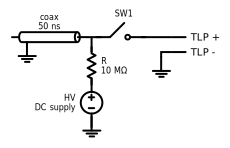
\includegraphics[width=\textwidth]{src/1/figures/tlp_concept.pdf}
  \caption{Minimal example of a \gls{tlp} system}
  \label{tlp_concept}
\end{figure}

% Characteristics of tlp systems
TLP systems constitute very well-controlled test generators.
The pulse is generated inside a shielded environment.
It is isolated from external radiated emissions and does not emit electromagnetic disturbances.
The characteristic impedance of 50\textOmega{} can be controlled up to the load, by using appropriate 50\textOmega{} cables and hardware.
Those properties result in clean and repeatable pulse waveforms without reflections.
The main features of the generated pulse are given in figure \ref{tlp_pulse}.

\begin{figure}[!h]
  \centering
  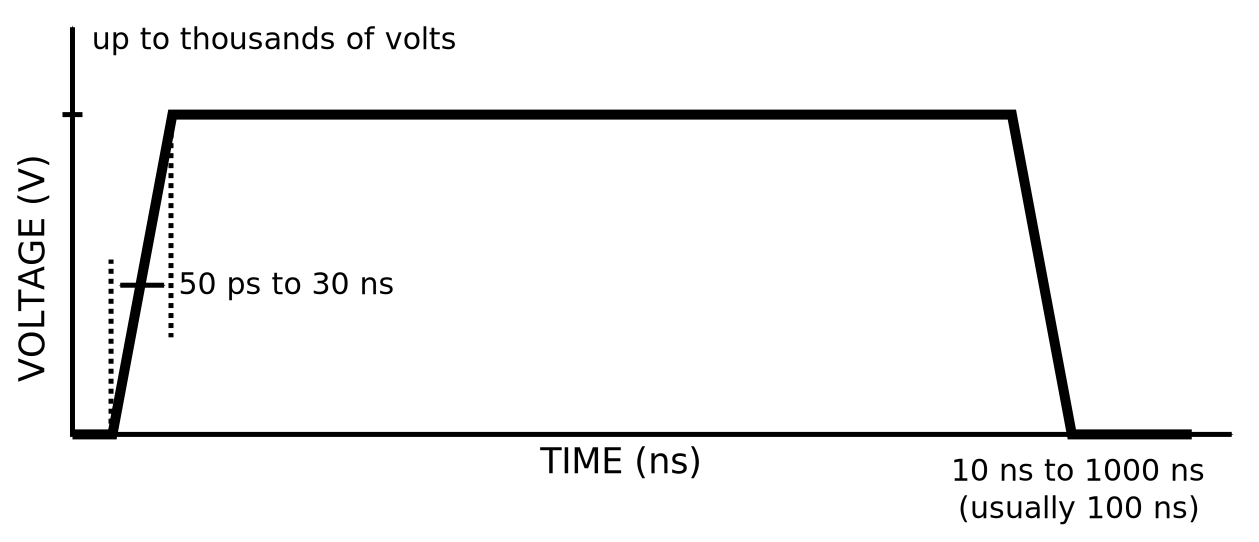
\includegraphics[width=\textwidth]{src/1/figures/tlp_pulse.pdf}
  \caption{Main characteristics of a \gls{tlp} pulse on a resistive load}
  \label{tlp_pulse}
\end{figure}

% Control over the pulse shape
The waveform parameters are completely controlled and easily tunable.
The charging voltage is set by the high-voltage source.
The pulse width can be increased or decreased by changing the length of the coaxial cable.
The risetime can be enforced with a 50\textOmega{} matched risetime filter \cite{cao-risetime-filter, gaussian-lpf}.
Unlike most filters, they are specifically designed to work by absorption and not by reflection.
They do not pollute the system with reflected waves.

\gls{tlp} generators can also be employed as a measurement tool.
Some configurations use Time-Domain Reflectometry (TDR) and others rely on more standard techniques for measuring electrical properties of a load.

% Principle of TDR for TLP
%TODO: Find TLP TDR reference, and non TDR TLP ref
Time-domain reflectometry is a measurement technique with a wide range of applications.
With TDR, it is possible to determine electrical properties of a device by observing reflected waveforms.
In this configuration, voltage and current measured at the output of the generator are equal to voltage and current waveforms inside the load.

\begin{figure}[!h]
  \centering
  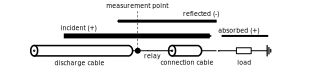
\includegraphics[width=\textwidth]{src/1/figures/tlp_pulse_superposition.pdf}
  \caption{TDR measurement with incident and reflected waves superposition}
  \label{fig:tlp-superposition}
\end{figure}

This is due to the superposition of the incident and reflected pulses during the discharge (see Fig. \ref{fig:tlp-superposition}).
When the relay is closed, an incident wave appears that propagates toward the load.
The impedance mismatch between the load and the connection cable forces a part of the incident power to reflect back.
The rest is absorbed and dissipated by the load.
This reflected wave corresponds to the difference between the incident power and the absorbed power, but with a negative sign.
At the measurement point, the incident wave and the reflected wave add up.
Eq. \ref{eq:tdr-tlp} explains how this sum is equal the value absorbed by the load, for the voltage.
Same equation applies for current.
In summary, the measured voltage and currents at the output of the TLP are equal to the voltage and current inside the load, when incident and reflected waves are sumperimposed.
An extensive analysis of \gls{tdr} \gls{tlp} is provided in \cite{phd-monnereau}.

\begin{equation}
V_{measured} = V_{incident} + V_{reflected} = V_{incident} + (- (V_{incident} - V_{absorbed})) = V_{absorbed}
\label{eq:tdr-tlp}
\end{equation}

% Explanation of a typical esd protection response
Fig. \ref{fig:typical-tlp-response} provides an example of a typical waveform generated by a \gls{tlp} injecting on an \gls{esd} protection.
The recording is done in a \gls{tdr} configuration.
Voltage and current waveforms usually exhibit two steps.
The first step is due to the connection cable that links the \gls{tlp} to the load (see previously Fig. \ref{tlp_concept}).
Delay \textDelta{}t\textsubscript{1} corresponds to the delay of the connection cable.
The ratio $V_{1}/I_{1}$ is equal to the characteristic impedance of the connection cable, usually 50\textOmega{}.
The second step is the response of the tested load.
The value $V_{2}/I_{2}$ is the quasi-static resistance of the load.
$V_{2}/I_{2}$ is a function of the \gls{tlp} charging voltage.
By averaging each waveform during a few tens of nanosecond, the current and voltage value of the load can be accurately sampled.

\begin{figure}[!h]
  \centering
  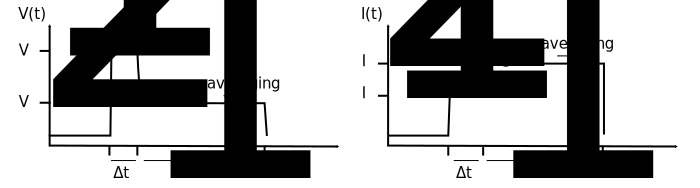
\includegraphics[width=\textwidth]{src/1/figures/tlp_response.pdf}
  \caption{TLP V(t) and I(t) example}
  \label{fig:typical-tlp-response}
\end{figure}

% Continue explanantion
The pulse ends when the main coaxial cable is fully discharged.
The pulse lasts twice the delay of the discharge cable.
At $t=0ns$ the relay is closed.
The cable starts discharging from the end closer to the relay.
The other end starts discharging only 50ns later because of the propagation delay.
It takes another 50ns delay for the discharge to completely propagate back to the relay side.
This explain why the pulse length is twice the coaxial cable delay.

% Main application of TLP is IV characterization
A very popular application of transmission line pulsers is the extraction of an $I(V)$ curve \ref{fig:iv-curve-extraction} from a set of pulses and measurements.
An $I(V)$ represents the current versus voltage response of a device.
They are called quasi-static because values are sampled during a short amount of time and cannot be entirely assimilated to a DC characterization.
They are extracted at much larger levels than the device can withstand in DC.
Quasi-static $I(V)$ curves are particularly useful for characterization of ESD protections \cite{TLPforESDProtectionCz}, that by nature work in transient regime and cannot be studied in DC.

\begin{figure}[!h]
  \centering
  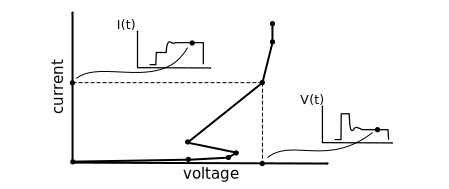
\includegraphics[width=0.9\textwidth]{src/1/figures/tlp_iv_curve.pdf}
  \caption{TLP-extracted I(V) characteristic example}
  \label{fig:iv-curve-extraction}
\end{figure}

% How are I(V) curves extracted
The $I(V)$ curve is extracted point after point.
Each point corresponds a voltage and current measured by averaging the transient waveforms during the second step.
A first pulse is injected, current and voltage are measured, and the coordinates of a first point are extracted.
Then the process is repeated and the charging voltage is incremented after each new point (Fig. \ref{fig:iv-curve-extraction}).
Depending on the kind of tested device, snapback responses can sometimes be measured.
A snapback response is a non-monotonous curve, where a single x-axis value (voltage) can correspond to multiple y-axis values (current).
Snapbacks are impossible to observe with a DC $I(V)$ characterization.
An example is provided in Fig. \ref{fig:iv-curve-extraction}.
Snapbacks are observed for devices with at least two different states of operation.
In the off-state, it acts as a high-value resistance and current increases very slowly when voltage gets higher.
When the device turns on, its resistance drops abruptly and becomes very small.
Currents suddenly increases and voltage falls.
This transistion corresponds to the discontinuity visible on the curve.

% Another application is the characterization of the robustness
TLPs are also commonly used for testing the robustness of systems and devices \cite{TLPthroubleshooting, LacrampeTransientImmunity}.
It is great for troubleshooting because the pulse and well repeatable.
A rectangular waveform is also more desirable for investigation, it simplifies the analysis.
However in some cases, it can be an issue for reproducing a failure observed with more time-varying waveforms like IEC 61000-4-2 \gls{\cite{iec61000-4-2}} described after.

% vf-tlp
A few variations of the TLP exist to cover edge cases and specific characterization requirements.
The very-fast \gls{TLP} (vf-TLP) is one of them.
It was designed by H. Gieser \cite{vf-tlp} to reproduce gate oxyde breakdown.
Basically, it is a TLP with a shorter pulse width, usually in the range of 1ns to 10 ns.

% vf-tlp for reflectometry
vf-TLP requires more advanced calibration techniques for measuring load current and voltage, and stronger constrains on the quality and bandwidth of test elements and measurement systems.
In this configuration, incident and reflected waves never sumperimpose and by default time-domain reflectometry cannot be employed as-is.
However, E. Grund adapted the technique to vf-TLP in \cite{vf-tlp-tdr}.
With this method, it is possible analyse and calculate the impedance of all elements between the generator and the load.

% Minor conclusion
To sum up, Transmission Line Pulsing is an extremely versatile and useful technique for the \gls{esd} field.
It is not considered a qualification tester though because it does not reproduce any real-world electrostatic discharge events.
Standards and other techniques dedicated to this task are described hereafter.

\subsection{ESD Gun (IEC 61000-4-2 / ISO 10605)}

% What is the goal of this test
IEC 61000-4-2 \cite{iec61000-4-2} and ISO 10605 \cite{iso10605} standards define a system-level test waveform and test generator to reproduce the discharge of a human body through an electronic device.
This test is used very extensively for qualification of products.
Fig. \ref{fig:picture-esd-gun} provides a picture of an \gls{esd} gun.
The gun is composed of a metallic discharge tip to inject the pulse.
The ground return is a long metallic ribbon a couple of meters long.
Depending on the test configuration, it is connected to the product ground or the earth.
Its shape impacts a lot recorded failure levels.
Historically, ESD gun were famous for lacking some reproducibility on test results \cite{hmm-uncertainty}.
They have largely improved since then although radiated emissions and shape of the ground return still remain a very large factor of variation and uncertainty \cite{gun-rf-uncertainty}.

\begin{figure}[!h]
  \centering
  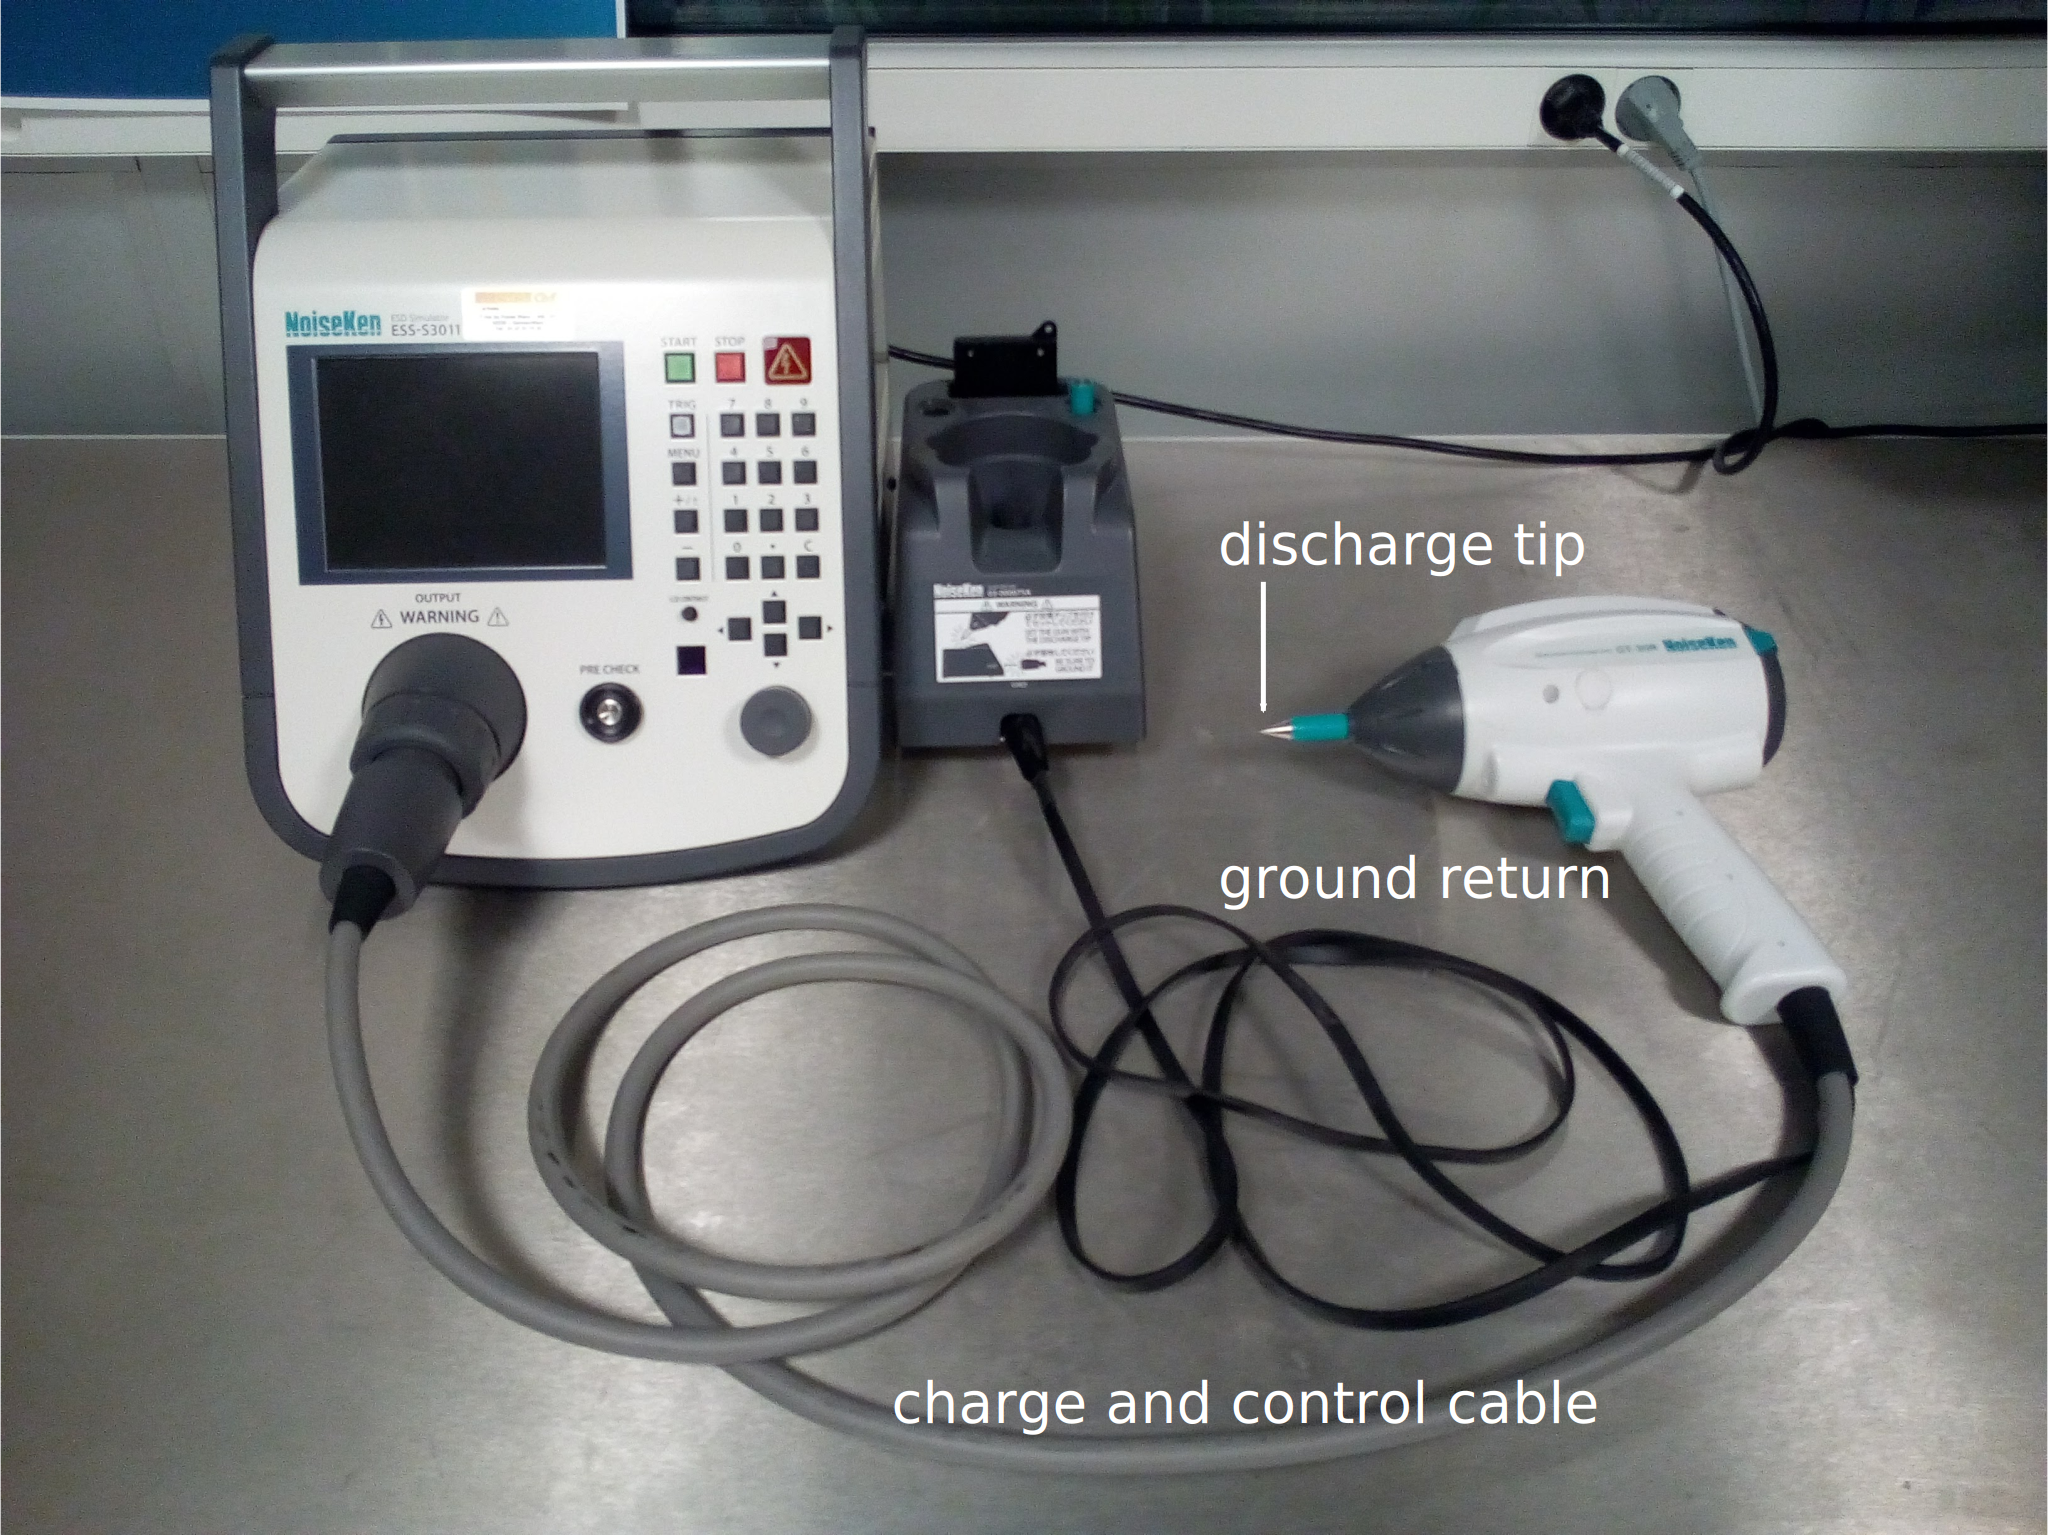
\includegraphics[width=0.3\textwidth]{src/1/figures/iec61000-4-2_picture.pdf}
  \caption{Picture of an ESD gun IEC 61000-4-2 compliant}
  \label{fig:picture-esd-gun}
\end{figure}

% Explain the waveform
%TODO: Why 2 ohms ?
Fig. \ref{iec_pulse} presents the main properties of the generated stress.
The standard defines this waveform for a 2\textOmega{} load.
The pulse starts by a fast peak with a $1ns$ risetime.
It is followed by a slower slope of smaller amplitude but longer duration of about $200ns$.
Voltage levels can reach 15kV peak and 30A of current.

\begin{figure}[!h]
  \centering
  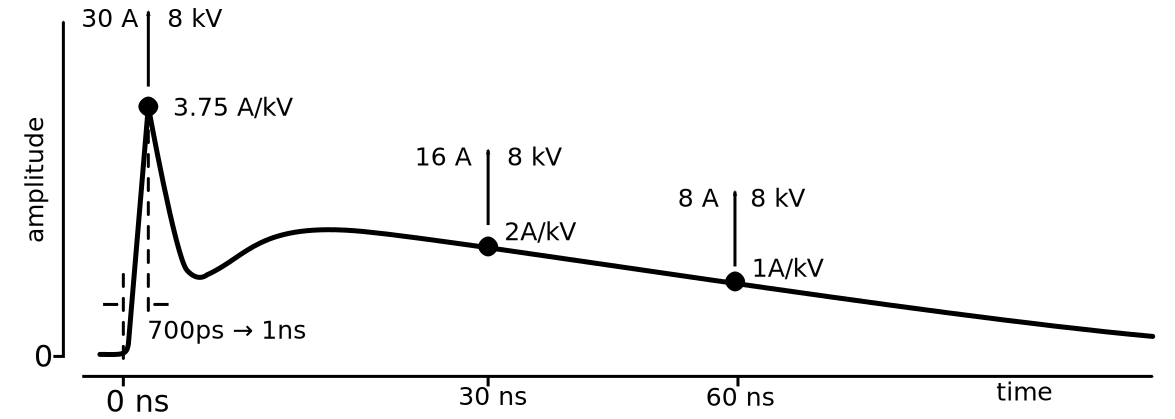
\includegraphics[width=\textwidth]{src/1/figures/iec61000-4-2_waveform.pdf}
  \caption{Main properties of an IEC 61000-4-2 pulse on a 2\textOmega\ resistive load}
  \label{iec_pulse}
\end{figure}

% How is the pulse generated
The generation of the ESD pulse is done with a 330\textOmega resistor and 150 pF capacitor discharge network.
The RC network alone though does not suffice to reproduce the waveform.
Parasitic devices play an important part in shaping the waveform.
Fig. \ref{fig:esd-gun-model} provides a physically-based ESD Gun model that helps understand the impact of parasitic devices.
This model was originally written by Chiu \cite{phd-chiu} and is referenced in the PhD thesis of N. Monnereau \cite{phd-monnereau}.
It adds an R\textsubscript{g}L\textsubscript{g}C\textsubscript{g} network to model the ground return.
A parasitic capacitance C\textsubscript{i} and series inductance L\textsubscript{i} model imperfections in the direct injection path.

\begin{figure}[!h]
  \centering
  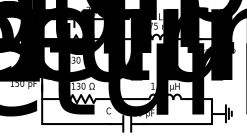
\includegraphics[width=0.3\textwidth]{src/1/figures/gun_model.pdf}
  \caption{ESD Gun model}
  \label{fig:esd-gun-model}
\end{figure}

% Talk about application fields
IEC 61000-4-2 \cite{iec61000-4-2} and ISO 10605 \cite{iso10605} are system-level standards, targeting different fields of application.
IEC 61000-4-2\cite{iec61000-4-2} standard targets consumer electronics.
ISO 10605\cite{iso10605} standard is intended for automotive equipment.
It defines additional pulse waveforms to cover a wider range of ESD events (See fig \ref{iso_pulse}).
Each pulse is generated with a different discharge network.
Instead of the usual 150pF - 330\textOmega{} values, all combinations with 330pF and 2k\textOmega{} are also possible.
% Talk about HMM
Finally, there is the \gls{hmm} \cite{hmm} specification.
It aims to adapt those system-level standards for component-level testing.
The pulse waveform remains identical, but a few modifications concerning the injection setup are proposed.
Most notably, the ground return of the gun is connected directly to the ground of the device, rather than the Earth.
The specification is standardized under ANSI/ESD SP5.6-2009 \cite{hmm}.

\begin{figure}[!h]
  \centering
  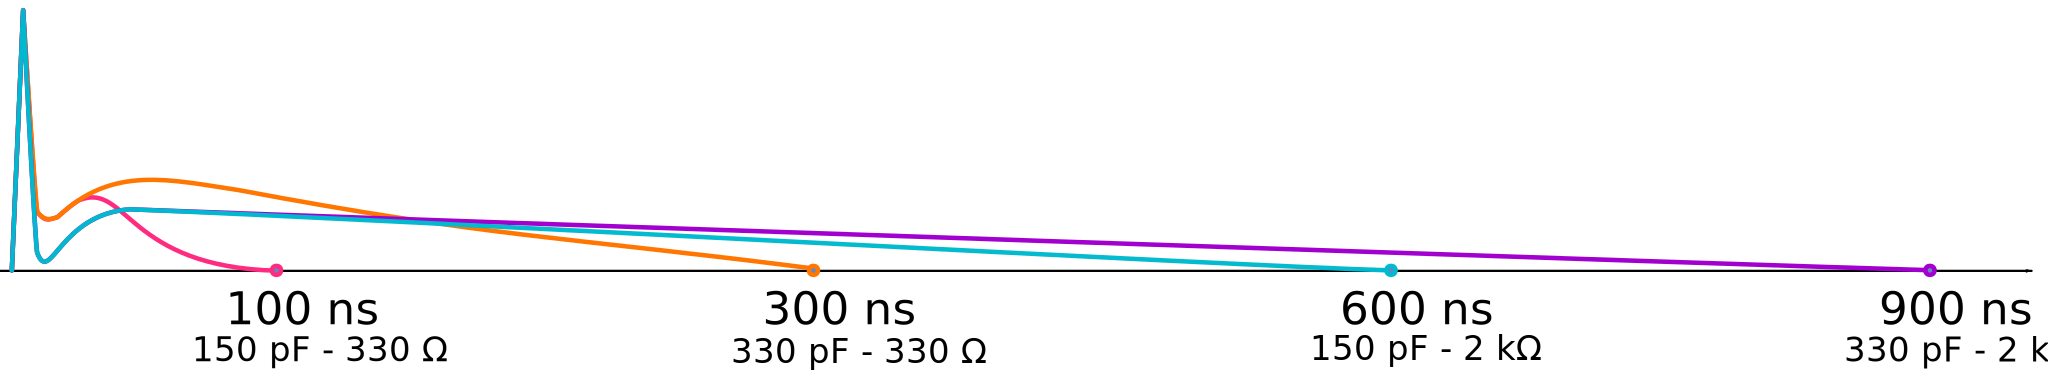
\includegraphics[width=\textwidth]{src/1/figures/iso10605_waveform.pdf}
  \caption{Waveforms defined in ISO 10605 standard on a 2\textOmega{} resistive load}
  \label{iso_pulse}
\end{figure}

%TODO: Annex F ISO 10605

ISO 10605 introduces the concept of performance classes for categorizing the robustness of powered-on electronic systems in operation against electrical disturbances.
Classes are defined from A to E, with A describing systems that are the more immune to the test.
Class E corresponds to the worst severity, where the electronic device did not survive the test.
Table \ref{tab:iso-class-a-levels} details the conditions specified for each class.

\begin{table}[!h]
\centering
\begin{tabular}{l|p{0.8\textwidth}}
Immunity class  & Definition   \\ \midrule
A  & All functions of a device or system perform as designed during and after exposure to interference.  \\ \midrule
B  & All functions of a device/system perform as designed during exposure; however, one or more of them may go beyond the specified tolerance. All functions return automatically to within normal limits after exposure is removed. Memory functions shall remain class A. \\ \midrule
C  & One or more functions of a device or system do not perform as designed during exposure but return automatically to normal operation after exposure is removed.   \\ \midrule
D  &  One or more functions of a device or system do not perform as designed during exposure and do not return to normal operation until exposure is removed and the device or system is reset by a simple “operator/use” action.   \\ \midrule
E   &  One or more functions of a device or system do not perform as designed during and after exposure and cannot be returned to proper operation without repairing or replacing the device or system.  \\
\bottomrule
\end{tabular}
\caption{Electronic systems performance classes from ISO10605}
\label{tab:iso-class-a-levels}
\end{table}

\subsection{ISO 7637-2}

% Where does this standard applies
ISO 7637-2\cite{iso7637-2} is an automotive standard for testing immunity of electronic devices against transient electrical disturbances.
It reproduces disturbances applied on supply lines, when the battery of a car is disconnected for instance.
This standard defines several waveforms.
Among them, pulses 2A and 3B are the closest to an electrostatic discharge.

% Pulse 2A - What is the goal of this pulse
Pulse 2A simulates the sudden disconnection of a load placed in parallel with the device under test.
In a car, it reproduces the switching of devices separated by inductive wiring harnesses.
When a load is abruptly switched off, the inductance opposes to the sudden interruption of current.
Instead of flowing through the load, the current is maintained and reported onto the \gls{dut} which can be damaged or disturbed in the process.
These events can be quite harmful with peak voltages above 50V during 50\textmu{}s.
This pulse can be an interesting testing waveform in the context of this entire document.
The characteristics of pulse 2A are given in fig. \ref{fig:iso_2a_pulse}.

\begin{figure}[!h]
  \centering
  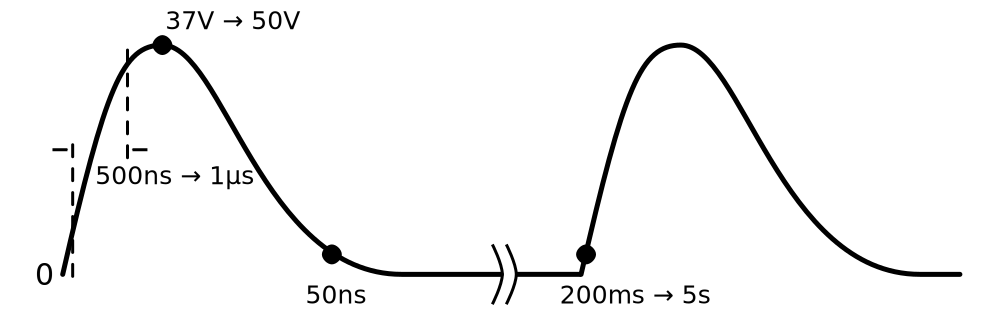
\includegraphics[width=0.7\textwidth]{src/1/figures/iso7637-2-2a.pdf}
  \caption{Waveform 2A defined in ISO 7637-2 standard on a 2\textOmega{} resistive load}
  \label{fig:iso_2a_pulse}
\end{figure}

% How is the pulse generated
%TODO: Is it 2 ohms ?
The ISO 7637-2 standard does not enforce how stress generators must be constructed or modelled.
A compliant generator can be implemented with a resistor-capacitor discharge network.
However, by tuning both values, it is rather straightforward to produce the standardized waveform on a 2\textOmega{} resistor.
It should be noted that the behavior of an RC network is quite different from an actual inductive load disconnection, but as long as the generated waveform is correct the generator is considered compliant.

\begin{figure}[!h]
  \centering
  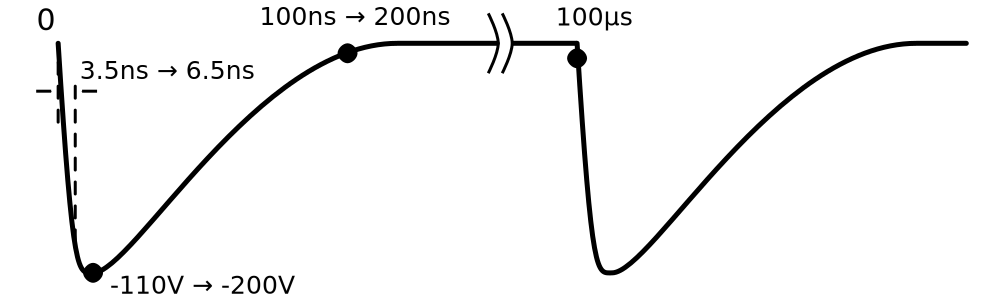
\includegraphics[width=0.7\textwidth]{src/1/figures/iso7637-2-3b.pdf}
  \caption{Waveform 3B defined in ISO 7637-2 standard on a 50\textOmega{} resistive load}
  \label{fig:iso_2b_pulse}
\end{figure}

% Pulse 3B - What is the goal of this pulse
Pulse 3B simulates the result of a switching process on a wiring harness, causing negative spikes on a \gls{dut}.
Its waveform is given in fig. \ref{fig:iso_2b_pulse}.
Compared to pulse 2a, this waveform has a shorter duration and risetime and a higher amplitude.
Interestingly, it is one of the rare \gls{esd} waveforms to be defined on a 50\textOmega{} load.

% Interest of this standard
A few papers \cite{is-iso7637-real, iso7637-2-new-automotive-reqs, robustness-esd-iso7637} studied the impact of those waveforms on integrated ESD protections.
Automotive equipment manufacturer are required to qualify products against ISO 7637-2, to guarantee they can survive the vicinity of other electrical modules in the car such as ignition systems.
Therefore, it is relevant to test functional robustness of devices against this standard.

% Modelling
The VDA FAT-AK30 working group on simulation of mixed-systems with VHDL-AMS \cite{fat-ak30} has worked on modelling all ISO 7637-2 generators. They have provided open-source models of all pulses defined in the standard, as part of the \textit{vdalib} library \cite{vdalib}.
For instance, VHDL-AMS model of pulse 3B is provided in Listing \ref{lst:iso-7637-pulse3b}.

\begin{code}
\inputminted[frame=single,firstline=157,lastline=228]{VHDL}{src/1/snippets/iso_7637_pulse3b.vhd}
\caption{Open-source VHDL-AMS model of ISO7637 pulse 3b - Copyright VDA/FAT}
\label{lst:iso-7637-pulse3b}
\end{code}


\subsection{IEC 61000-4-4}

% Where does this standard applies - scope
The IEC 61000-4-4 standard \cite{iec61000-4-4}, also called burst test, defines an electrical fast transient for \gls{esd} testing.
It defines a test waveform, generator and procedures for assessing susceptibility of electronic devices subjected to transient disturbances such as interruption of inductive loads and relay contact bounce.
It concerns all kinds of inputs such as supply, signal and control lines.
This standard applies is not focused on any specific field of application.

% What is the pulse
The defined waveform is a double exponential pulse \ref{fig:iec_4_4_pulse} with a width of 50ns at 50\% of the peak amplitude.
Risetime is comprised between 3.5ns and 6.5ns.
It is defined for a 50\textOmega{} load, with a pulse period of 15ms and a burst period of 300ms.

\begin{figure}[!h]
  \centering
  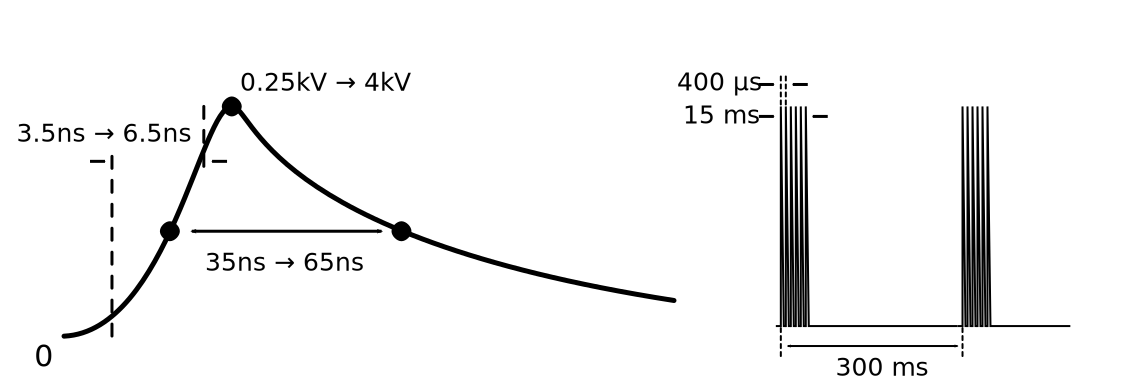
\includegraphics[width=\textwidth]{src/1/figures/iec61000-4-4_waveform.pdf}
  \caption{IEC 61000-4-4 waveform on a 50\textOmega{} resistive load}
  \label{fig:iec_4_4_pulse}
\end{figure}

% How is the pulse generated
The standard defines a circuit diagram for the generator (Fig \ref{fig:iec_4_4_generator}).
The discharge is produced by a resistor-capacitor R\textsubscript{C}-C\textsubscript{C} network and initiated by a spark-gap.
A spark-gap consists in two conductive tips separated by a gap.
When voltage accross the gap becomes superior to the breakdown voltage, a spark appears and resistance of the spark gap suddenly drops, allowing discharge current to flow through.
In Fig. \ref{fig:iec_4_4_generator}, R\textsubscript{s}, R\textsubscript{m} and C\textsubscript{d} shape the waveform.
R\textsubscript{s} defines the duration of the pulse, R\textsubscript{m} performs an impedance matching and C\textsubscript{d} act as a \gls{dc} block.
The generator's output is a coaxial plug to prevent radiated emission during the discharge.

\begin{figure}[!h]
  \centering
  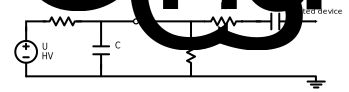
\includegraphics[width=0.8\textwidth]{src/1/figures/iec61000-4-4_diagram.pdf}
  \caption{IEC 61000-4-4 generator circuit diagram}
  \label{fig:iec_4_4_generator}
\end{figure}

% Injection method - capacitive coupling clamp
A particular injection method for powered lines called a \texit{capacitive coupling clamp} (Fig. \ref{fig:iec_4_4_clamp}) is defined in this standard.
This injection system is interesting for performing repeatable injection into powered supply lines.
The clamp is constituted of two large metallic plates.
The upper plate has the shape of of a tunnel, where the wires receiving go through.
The discharge is injected in the upper plates.
The bottom plate is connected to the ground of the discharge generator.
Thanks to this design, the shape of the wires and the entire setup is well controlled.
Although originally designed to work with the IEC 61000-4-4 waveform, the capacitive coupling clamp accepts coaxial cables and any kind of stress generator can be employed instead.

\begin{figure}[!h]
  \centering
  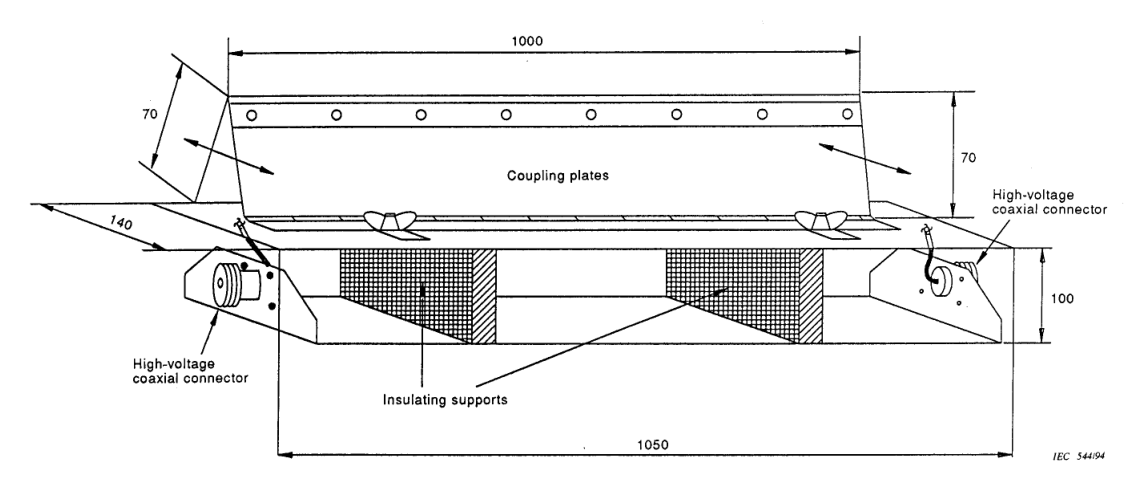
\includegraphics[width=0.8\textwidth]{src/1/figures/iec61000-4-4_clamp.png}
  \caption{IEC 61000-4-4 capacitive coupling clamp}
  \label{fig:iec_4_4_clamp}
\end{figure}

\subsection{IEC 62215 standard}

% Where does this standard applies - scope
The IEC 62215 standard \cite{iec62215} defines a method for measuring the immunity of an integrated circuit to conducted electrical transient disturbances.
It specifically targets testing of integrated circuits in operation.
Instead of specifying test pulses, this standard defines a way to inject stresses suitable for integrated circuits.
For automotive devices, the standard specifies the use of waveforms from ISO 7637-2 \cite{iso7637-2}.
IEC 61000-4-4 \cite{iec61000-4-4} or IEC 61000-4-5 are required for industrial and consumer applications.
Ultimately, the goal is to understand and classify interactions between a conducted disturbance and performance degradation induced in integrated circuits.
The test method ressembles the \gls{dpi} technique defined in IEC 62132-4 \cite{iec62132-4}.
The \gls{dpi} standard focuses on frequency domain immunity, while this standard tests time-domain immunity.

% How is the pulse generated
Disturbances are applied to the \gls{ic} pins via a coupling network, that isolates the stress generator and the \gls{dc} supply from one another.
A typical pin injection setup is given in Fig. \ref{fig:iec62215_setup}.

\begin{figure}[!h]
  \centering
  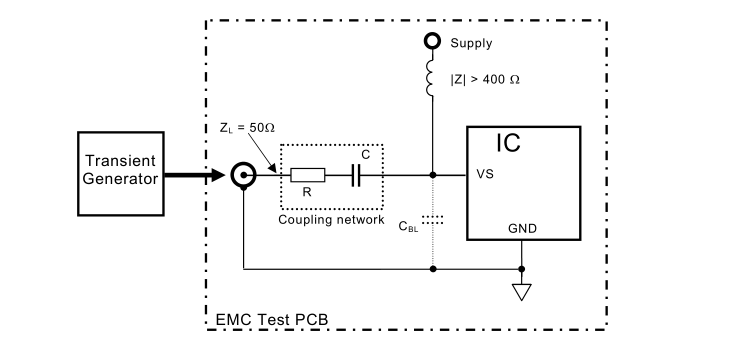
\includegraphics[width=0.9\textwidth]{src/1/figures/iec62215_setup.png}
  \caption{Typical injection setup via a coupling network}
  \label{fig:iec62215_setup}
\end{figure}

% Talk about immunity classes
%TODO
Beyond test setup and waveforms, the standard defines immunity classes (see Table \ref{tab:class-a-levels}) to categorize the behavior of integrated circuits exposed to disturbances.
It is a direct adaptation of performance classes defined in Annex B of ISO10605 and presented previously in Table \ref{tab:iso-class-a-levels}.
Classes range from A to E.
A describes devices that are completely unaffected by the testing procedure and maintain their entire functionnality.
B describes a short time degration of internal signals. It is not applicable for integrated circuits, where internal signals are most of the time not accessible.
C is identical to A, with the difference that failures can occur internally inside the chip, as long as they remain internal to the circuit and do not affect the final application.
Finally, D and E describe actual cases of failure, with E representing a hard-failure.

\begin{table}[!h]
\centering
\begin{tabular}{l|p{0.8\textwidth}}
Immunity class  & Definition   \\ \midrule
A\textsubscript{IC}   & All monitored functions of the IC perform within the defined tolerances during and after exposure to disturbance.      \\ \midrule
B\textsubscript{IC}   & Short time degradation of on or more monitored signals during exposure to disturbance is not evaluable for IC only. Therefore this classification is not applicable for ICs. \\ \midrule
C\textsubscript{IC}   & All monitored functions of the IC are within the defined tolerances before and after exposure to disturbance.        \\ \midrule
D\textsubscript{IC}   &  At least one monitored function of the IC does not perform within the defined tolerances during exposure and does not return to normal operation by itself. The IC returns to normal operation by simple action (e.g. reset).   \\ \midrule
E\textsubscript{IC}   &  At least one monitored function of the IC does not perform within the defined tolerances after exposure and can not be returned to proper operation.  \\
\bottomrule
\end{tabular}
\caption{IC performance classes from IEC62215}
\label{tab:class-a-levels}
\end{table}
